\documentclass[10pt]{jsarticle}
\usepackage{cases}
\usepackage{bm}
\usepackage[dvipdfmx]{graphicx}
\begin{document}
\begin{center}
{\LARGE 音声情報処理 レポート}\\
2017/11/7\\
 27115126 CSb 長谷川達也\\
\end{center}
\clearpage
\section{}
与えれたデータを用いて、シングルテンプレートマッチングで識別を行った結果を以下の表にまとめる。\\
\begin{table}[h]
\centering
\begin{tabular}{|cc||ccccc|rrr|} \hline
\multicolumn{2}{|c||}{} 	& \multicolumn{5}{c|}{識別結果(個数)}	& 正解	& 誤り		& 正解率\\
\multicolumn{2}{|c||}{} 	& a & i & u & e & o 			& (個数) 	& (個数) 	& (\%) \\ \hline \hline
	 	& a 	    	& 2 & 0 & 4 & 0 & 0 			& 2 		& 4 		& 33.3\\
		& i 		& 0 & 1 & 5 & 0 & 0 			& 1 		& 5 		& 16.7\\
テストデータ 	& u 		& 0 & 0 & 5 & 0 & 1 			& 5 		& 1 		& 83.3\\
	 	& e 		& 0 & 1 & 3 & 1 & 1 			& 1 		& 5 		& 16.7\\
	 	& o 		& 0 & 0 & 3 & 0 & 3 			& 3 		& 3 		& 50.0\\ \hline \hline
\multicolumn{7}{|r|}{全体} 						& 12		& 18		& 40.0\\ \hline
\end{tabular}
\end{table}
\par
各母音を識別するために学習させたデータがそれぞれ1つだけであったため、テストデータにうまく適合できず、誤った母音として判断されている
もののほうが多くなってしまっている。
\\ \\
また、各学習データにおいて抽出したケプストラムに対応するスペクトルをプロットしたものを以下に示す。
\begin{itemize}
\item a\\ \\
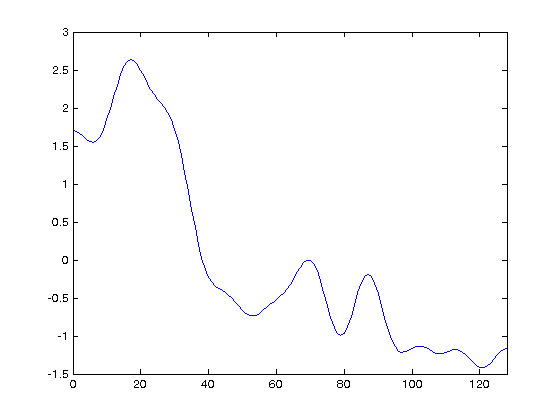
\includegraphics[width = 6cm]{result_textures/a_cepstrum.png}
\item i\\ \\
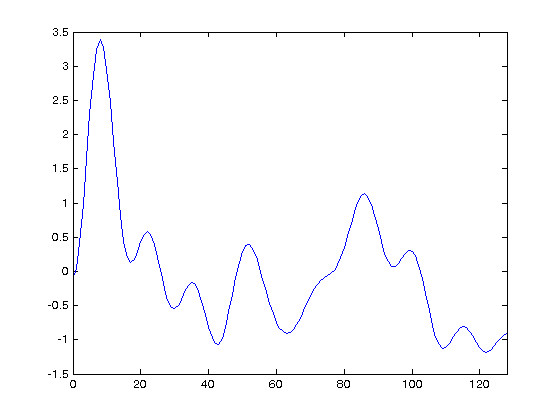
\includegraphics[width = 6cm]{result_textures/i_cepstrum.png}
\clearpage
\item u\\ \\
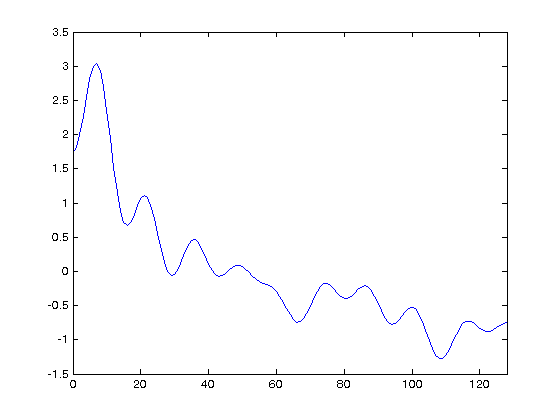
\includegraphics[width = 6cm]{result_textures/u_cepstrum.png}
\item e\\ \\
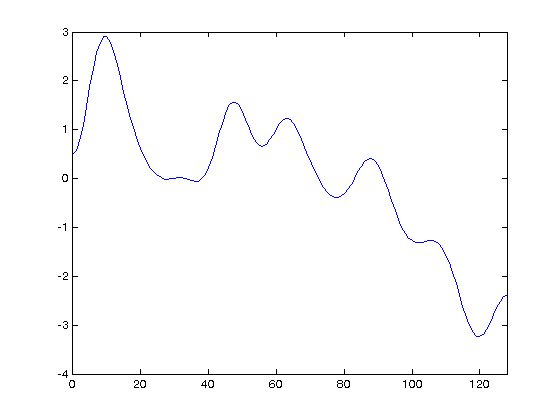
\includegraphics[width = 6cm]{result_textures/e_cepstrum.png}
\item o\\ \\
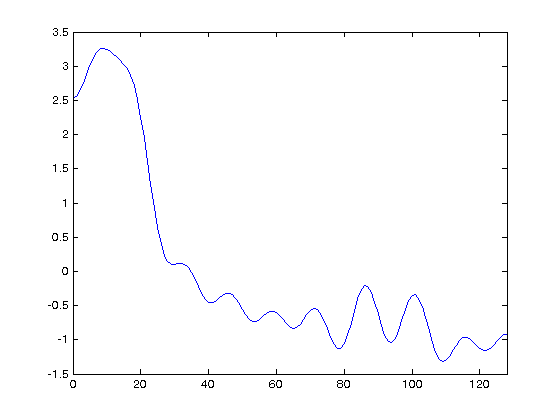
\includegraphics[width = 6cm]{result_textures/o_cepstrum.png}
\end{itemize}
\clearpage
スペクトルの形状を比較してみると、以下のような違いがあげられる。
\begin{itemize}
\item aとoは波の数やスペクトルの形状において似ているとみることができ、二つの母音は周期が似ていると考えられる。\\

\item uとeは直線的にみると、同じように右下がりになっているように見ることができるが、uのほうが急に振れ幅が減っている
のが見て取れる。\\

\item iは一度振れ幅が下がった後もう一度上がっている唯一の音であることが見て取れるので、母音の中では周期が
一番短いのではと予測できる。\\
\end{itemize}
また、さきほどの識別において識別誤りを起こしたデータをそれぞれ1つづつピックアップして、比較してみる。
\begin{itemize}
\item a\\
\item i\\
\item u\\
\item e\\
\item o\\
\end{itemize}
\section{}
各母音の識別率を上げるために、今回はシングルテンプレートマッチングにおいて学習データの数を増やして、それらで得られたパラメータの
平均を用いて識別を行ってみた。その結果を以下の表にまとめる。
\begin{table}[h]
\centering
\begin{tabular}{|cc||ccccc|rrr|} \hline
\multicolumn{2}{|c||}{} 	& \multicolumn{5}{c|}{識別結果(個数)}	& 正解	& 誤り		& 正解率\\
\multicolumn{2}{|c||}{} 	& a & i & u & e & o 			& (個数) 	& (個数) 	& (\%) \\ \hline \hline
	 	& a 	    	& 6 & 0 & 0 & 0 & 0 			& 6 		& 0 		& 100\\
		& i 		& 0 & 3 & 3 & 0 & 0 			& 3 		& 3 		& 50.0\\
テストデータ 	& u 		& 0 & 0 & 6 & 0 & 0 			& 6 		& 0 		& 100\\
	 	& e 		& 0 & 1 & 0 & 5 & 0 			& 5 		& 1 		& 83.3\\
	 	& o 		& 2 & 0 & 0 & 0 & 4 			& 4 		& 2 		& 66.7\\ \hline \hline
\multicolumn{7}{|r|}{全体} 						& 24		& 6		& 80.0\\ \hline
\end{tabular}
\end{table}
学習データが各母音において1つだった時に比べると、識別率は倍になっているのがわかる。サンプル数が増えて、ある程度いろいろなパターンの学習ができたためであると考えられる。
\end{document}